\section{1174017 - Muh. Rifky Prananda}
\subsection{Soal Teori}
\begin{enumerate}
	\item Jelaskan apa itu klasifikasi teks, sertakan gambar ilustrasi buatan sendiri.
	\hfill\break
	Klasifikasi teks adalah suatu proses untuk menkategorikan atau mengelompokkan teks atau dokumen ke dalam label tertentu.
	\hfill\break
	Contoh:
	\hfill\break
	Spam Filtering = mengklasifikasikan email atau pesan ke dalam class spam dan bukan spam.
	\hfill\break
	\begin{figure}[H]
	\centering
		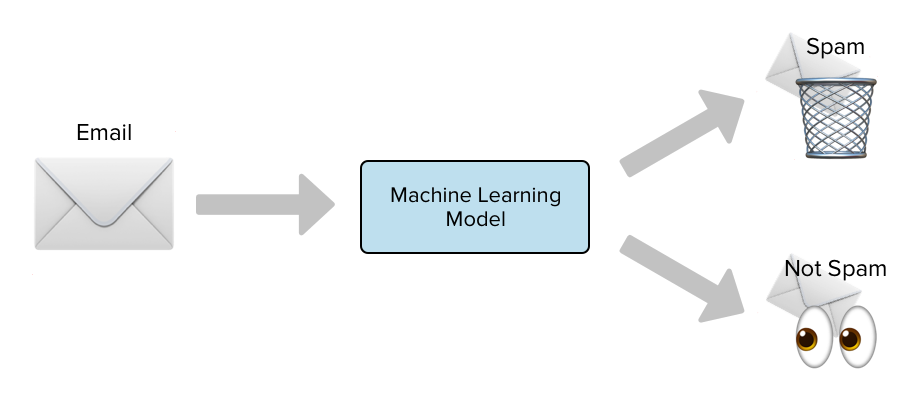
\includegraphics[width=8 cm]{figures/1174017/chapter4/soalteori/1.PNG}
	\end{figure}

	\item Jelaskan mengapa klasifikasi bunga tidak bisa menggunakan machine learning, sertakan ilustrasi sendiri.
	\hfill\break
	Klasifikasi bunga tidak bisa menggunakan machine learning karena setiap spesies bunga yang sama memiliki ukuran yang berbeda. Sehingga ukuran bunga tersebut tidak bisa menjadi patokan dalam mengklasifikasikan spesies bunga.
	\hfill\break
	Contoh:
	\hfill\break
	Pada dataset iris, untuk membedakan spesies bunga iris memerlukan panjang petal, lebar petal, panjang sepal, dan lebar sepal. Belum tentu yang memiliki panjang petal, lebar petal, panjang sepal, dan lebar sepal sepersekian termasuk spesies bunga iris saja.

	\item Jelaskan bagaimana teknik pembelajaran mesin pada teks pada kata-kata yang digunakan di youtube, jelaskan arti per atribut data csv dan sertakan ilustrasi buatan sendiri.
	
	Teknik machine learning yang dipakai pada teks yang digunakan di youtube bisa menggunakan bag of words dan random forest. Bag of words adalah proses mengubah teks menjadi vektor dengan panjang tetap dengan cara menghitung berapa kali setiap kata itu muncul. Random forest (RF) adalah suatu algoritma yang digunakan pada klasifikasi data dalam jumlah yang besar. Klasifikasi random forest dilakukan melalui penggabungan pohon (tree) dengan melakukan training pada sampel data yang dimiliki.\\
	Atribut yang ada pada file csv Youtube01-Psy diantaranya, COMMENT\_ID, AUTHOR, DATE, CONTENT, CLASS.
	\begin{itemize}
		\item COMMENT\_ID : merupakan key unik yang membedakan komen lainnya.
		\item AUTHOR : merupakan penulis dari komen tersebut.
		\item DATE : merupakan waktu dari komen tersebut dipublikasikan.
		\item CONTENT : merupakan isi komentarnya.
		\item CLASS : merupakan klasifikasi dari komennya.
	\end{itemize}

	\item Jelaskan apa yang dimaksud vektorisasi data.
	
	Vektorisasi data adalah mengubah data menjadi vektor berdasarkan ketentuan yang telah ditetapkan.
	

	\item Jelaskan apa itu bag of words dengan kata-kata yang sederhana dan ilustrasi sendiri.
	
	Bag of words adalah proses mengubah teks menjadi vektor dengan panjang tetap dengan cara menghitung berapa kali setiap kata itu muncul.
	\hfill\break
	Contoh:
	\hfill\break
	Misalkan kita mempunyai 3 dokumen:
	\begin{itemize}
		\item the cat sat
		\item the cat sat in the hat
		\item the cat with the hat
	\end{itemize}
	Temukan kosakata yang ada pada 3 dokumen itu. Kosakata yang ditemukan, diantaranya: the, cat, sat, in, the, hat, and with.
	\hfill\break
	Kemudian kita vektorisasi dokumen tersebut dengan cara menghitung berapa kali kata tersebut muncul.
	\begin{figure}[H]
	\centering
		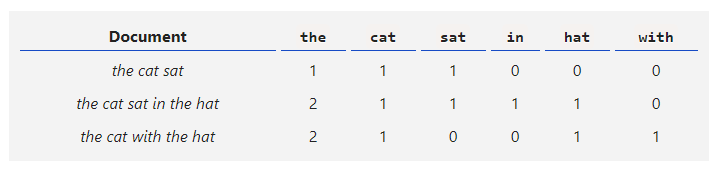
\includegraphics[width=8 cm]{figures/1174017/chapter4/soalteori/3.PNG}
	\end{figure}

	Hasilnya seperti ini:
	\begin{itemize}
		\item the cat sat: \[1, 1, 1, 0, 0, 0\]
		\item the cat sat in the hat: \[2, 1, 1, 1, 1, 0\]
		\item the cat with the hat: \[2, 1, 0, 0, 1, 1\]
	\end{itemize}

	\item Jelaskan apa itu TF-IDF, ilustrasikan dengan gambar sendiri.
	
	Term Frequency — Inverse Document Frequency atau TF — IDF adalah suatu metode algoritma yang berguna untuk menghitung bobot setiap kata yang umum digunakan. Metode ini juga terkenal efisien, mudah dan memiliki hasil yang akurat. Metode ini akan menghitung nilai Term Frequency (TF) dan Inverse Document Frequency (IDF) pada setiap token (kata) di setiap dokumen dalam korpus. Secara sederhana, metode TF-IDF digunakan untuk mengetahui berapa sering suatu kata muncul di dalam dokumen.
	
	TF (Term Frequency) adalah frekuensi dari kemunculan sebuah term dalam dokumen yang bersangkutan. Semakin besar jumlah kemunculan suatu term (TF tinggi) dalam dokumen, semakin besar pula bobotnya atau akan memberikan nilai kesesuaian yang semakin besar.

	IDF (Inverse Document Frequency) merupakan sebuah perhitungan dari bagaimana term didistribusikan secara luas pada koleksi dokumen yang bersangkutan. IDF menunjukkan hubungan ketersediaan sebuah term dalam seluruh dokumen. Semakin sedikit jumlah dokumen yang mengandung term yang dimaksud, maka nilai IDF semakin besar.
	\hfill\break
	Rumus:
	\hfill\break
	\begin{figure}[H]
	\centering
		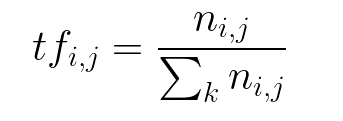
\includegraphics[width=8 cm]{figures/1174017/chapter4/soalteori/2-1.PNG}
	\end{figure}
	\hfill\break
	\begin{figure}[H]
	\centering
		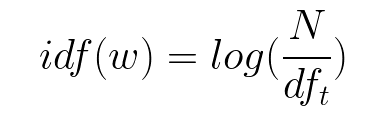
\includegraphics[width=8 cm]{figures/1174017/chapter4/soalteori/2-2.PNG}
	\end{figure}
	\hfill\break
	Contoh:
	\hfill\break
	\begin{figure}[H]
	\centering
		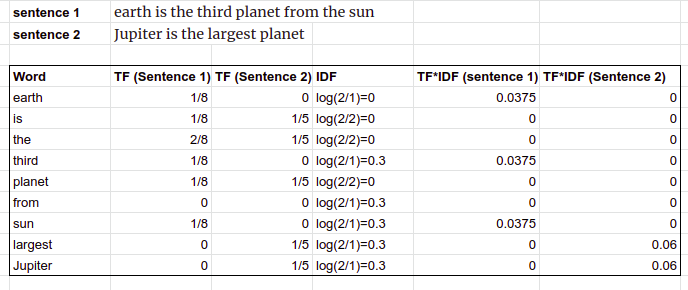
\includegraphics[width=8 cm]{figures/1174017/chapter4/soalteori/2.PNG}
	\end{figure}

\end{enumerate}

\subsection{Praktek Program}
\begin{enumerate}
	\item buat aplikasi sederhana menggunakan pandas, buat data dummy format csv sebanyak 500 baris dan melakukan load ke dataframe panda. jelaskan arti setiap baris kode yang dibuat(harus beda dengan teman sekelas)
	\lstinputlisting[firstline=2, lastline=3]{src/1174017/chapter4/praktek1.py}
	\hfill\break
	\begin{figure}[H]
	\centering
		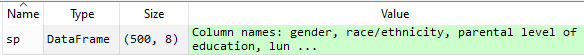
\includegraphics[width=8 cm]{figures/1174017/chapter4/soalpraktek/1-1-1.PNG}
	\end{figure}
	\item dari dataframe tersebut dipecah menjadi dua dataframe yaitu 450 row pertama dan 50 row sisanya (harus beda dengan teman sekelas)
	\lstinputlisting[firstline=5, lastline=5]{src/1174017/chapter4/praktek1.py}
	\hfill\break
	\begin{figure}[H]
	\centering
		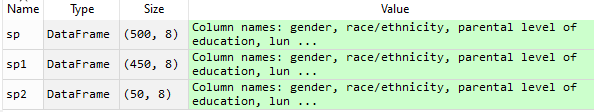
\includegraphics[width=8 cm]{figures/1174017/chapter4/soalpraktek/1-1-2.PNG}
	\end{figure}
	\item pratekkan vektorisasi dan klasifikasi dari data (NPM mod 4, jika 0 maka katty perry, 1 LMFAO, 2 Eminem, 3 Shakira) dengan Decission Tree. Tunjukkan keluarannya dari komputer sendiri dan artikan maksud setiap luaran yang didapatkan.
	\hfill\break
	\begin{figure}[H]
	\centering
		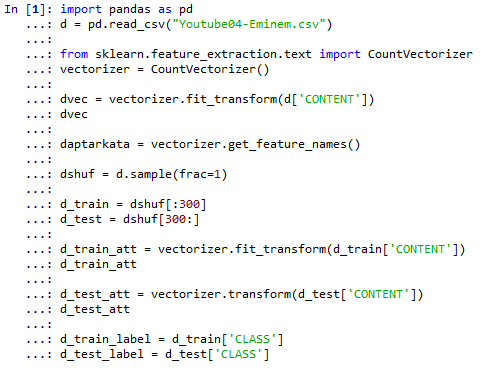
\includegraphics[width=8 cm]{figures/1174017/chapter4/soalpraktek/1-1.PNG}
	\end{figure}
	Vektorisasi data content dari file Youtube04\_Eminem.CSV
	\hfill\break
	\begin{figure}[H]
	\centering
		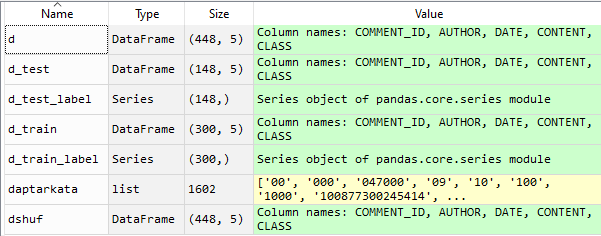
\includegraphics[width=8 cm]{figures/1174017/chapter4/soalpraktek/1-2.PNG}
	\end{figure}
	\item Cobalah klasifikasikan dari data vektorisasi yang di tentukan di nomor sebelumnya dengan klasifikasi SVM. Tunjukkan keluarannya dari komputer sendiri dan artikan maksud setiap luaran yang didapatkan.
	\hfill\break
	\begin{figure}[H]
	\centering
		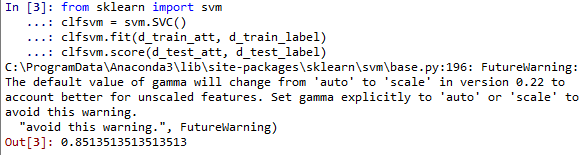
\includegraphics[width=8 cm]{figures/1174017/chapter4/soalpraktek/3-1.PNG}
	\end{figure}
	Hasil akurasi dari klasifikasi SVM.
	\item Cobalah klasifikasikan dari data vektorisasi yang di tentukan di nomor sebelumnya dengan klasifikasi Decission Tree. Tunjukkan keluarannya dari komputer sendiri dan artikan maksud setiap luaran yang didapatkan.
	\hfill\break
	\begin{figure}[H]
	\centering
		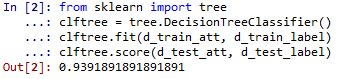
\includegraphics[width=8 cm]{figures/1174017/chapter4/soalpraktek/2-1.PNG}
	\end{figure}
	Hasil akurasi dari klasifikasi Decission Tree.
	\item Plotlah confusion matrix dari praktek modul ini menggunakan matplotlib. Tunjukkan keluarannya dari komputer sendiri dan artikan maksud setiap luaran yang didapatkan.
	\hfill\break
	\begin{figure}[H]
	\centering
		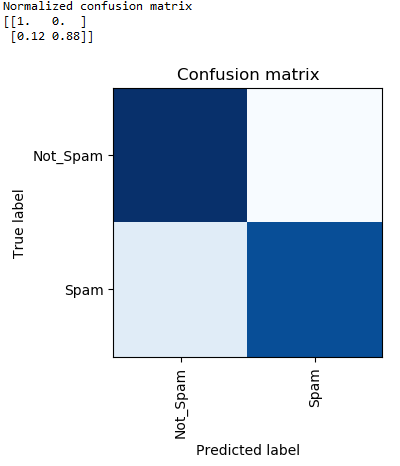
\includegraphics[width=8 cm]{figures/1174017/chapter4/soalpraktek/4-1.PNG}
	\end{figure}
	Plot confusion matrix dari klasifikasi Decission Tree.
	\hfill\break
	\begin{figure}[H]
	\centering
		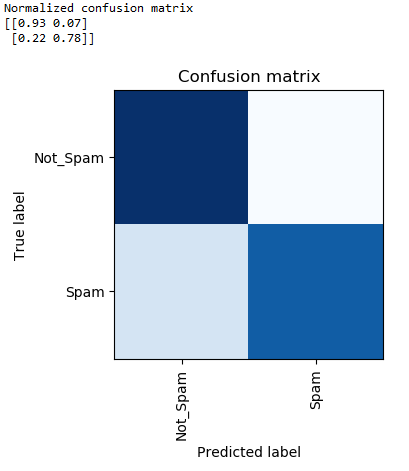
\includegraphics[width=8 cm]{figures/1174017/chapter4/soalpraktek/4-2.PNG}
	\end{figure}
	Plot confusion matrix dari klasifikasi SVM
	\item jalankan program cross validaiton pada bagian teori bab ini. Tunjukkan keluarannya dari komputer sendiri dan artikan maksud setiap luaran yang didapatkan.
	\hfill\break
	\begin{figure}[H]
	\centering
		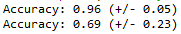
\includegraphics[width=8 cm]{figures/1174017/chapter4/soalpraktek/5-1.PNG}
	\end{figure}
	Hasil cross validation dari klasifikasi Decission Tree dan klasifikasi SVM.
	\item Buatlah program pengamatan komponen informasi pada bagian teori bab ini. Tunjukkan keluarannya dari komputer sendiri dan artikan maksud setiap luaran yang didapatkan.
	\item \hfill\break
	\begin{figure}[H]
	\centering
		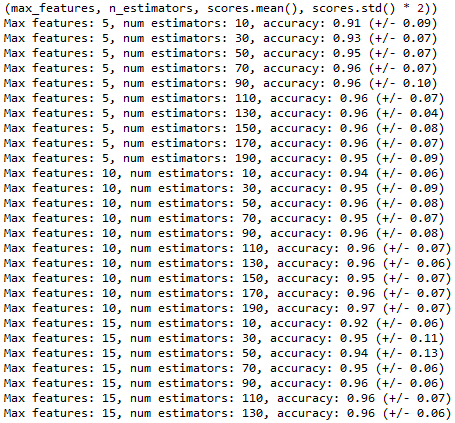
\includegraphics[width=8 cm]{figures/1174017/chapter4/soalpraktek/6-1.PNG}
	\end{figure}
	Hasil dari pengamatan komponen informasi menggunakan klasifikasi Random Forest.
\end{enumerate}

\subsection{Penanganan Error}
\begin{enumerate}
	\item Skrinsut error.
	\begin{itemize}
		\item Name Error
		\hfill\break
		\begin{figure}[H]
			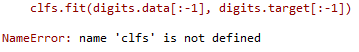
\includegraphics[width=8 cm]{figures/1174017/chapter1/error/err3.PNG}
			\centering
			\caption{Name Error.}
		\end{figure}
		\item Import Error
		\hfill\break
		\begin{figure}[H]
			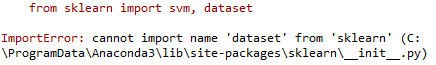
\includegraphics[width=8 cm]{figures/1174017/chapter1/error/err1.PNG}
			\centering
			\caption{Import Error.}
		\end{figure}
		\item Value Error
		\hfill\break
		\begin{figure}[H]
			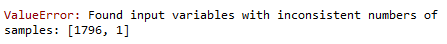
\includegraphics[width=8 cm]{figures/1174017/chapter1/error/err2.PNG}
			\centering
			\caption{Value Error.}
		\end{figure}
		\item Syntax Error
		\hfill\break
		\begin{figure}[H]
			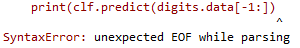
\includegraphics[width=8 cm]{figures/1174017/chapter1/error/err4.PNG}
			\centering
			\caption{Syntax Error.}
		\end{figure}
	\end{itemize}
	\item Tuliskan kode eror dan jenis errornya.
	\begin{itemize}
		\item Name Error
		\hfill\break
		Name Error adalah exception yang terjadi saat syntax melakukan eksekusi terhadap local name atau global name yang tidak terdefinisi.
		\item Import Error
		\hfill\break
		Import Error adalah exception yang terjadi saat syntax melakukan import terhadap library yang tidak terdefinisi.
		\item Value Error
		\hfill\break
		Value Error adalah exception yang terjadi saat syntax memiliki nilai yang tidak valid.
		\item Syntax Error
		\hfill\break
		Syntax Error adalah exception yang terjadi saat ada kesalahan dalam mengetikkan syntax.
	\end{itemize}
	\item Solusi pemecahan masalah error tersebut.
	\begin{itemize}
		\item Name Error
		\hfill\break
		Solusinya adalah memastikan variabel atau function yang dipanggil ada atau tidak salah ketik.
		\item Import Error
		\hfill\break
		Solusinya adalah memastikan library yang dipanggil ada atau tidak salah ketik.
		\item Value Error
		\hfill\break
		Solusinya adalah memastikan nilai yang diinputkan valid.
		\item Syntax Error
		\hfill\break
		Solusinya adalah memastikan syntax yang diketik tidak salah ketik.
	\end{itemize}
\end{enumerate}

\subsection{Bukti Tidak Plagiat}
\begin{figure}[H]
	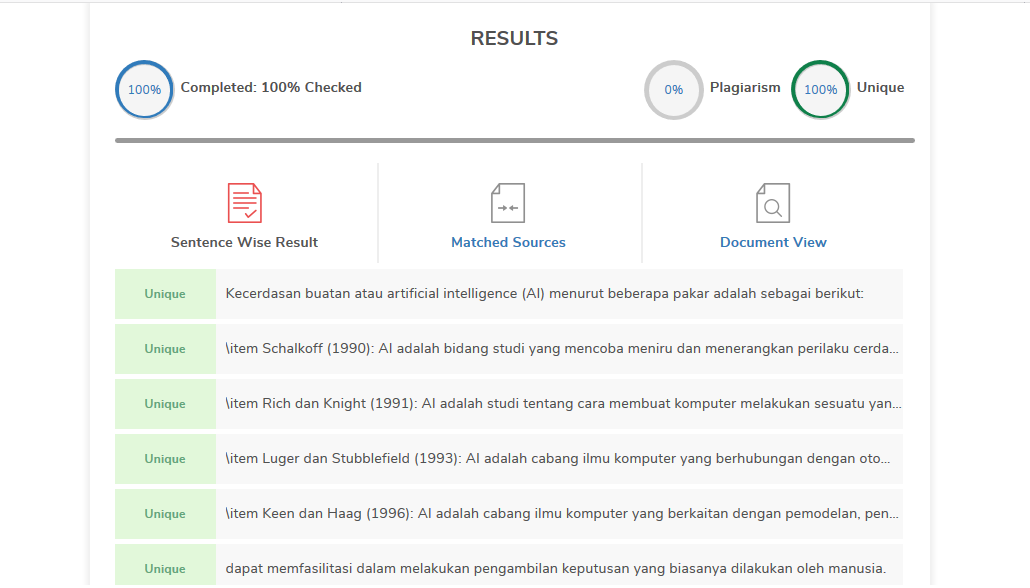
\includegraphics[width=8 cm]{figures/1174017/chapter1/plagiat.png}
	\centering
	\caption{Bukti Tidak Plagiat.}
\end{figure}